%! Mode:: "TeX:UTF-8"
%! TEX program = xelatex
\PassOptionsToPackage{quiet}{xeCJK}
\documentclass[withoutpreface,notoc]{cumcmthesis}

% === 建议在此处加载 cls 文件未包含的、个人需要的宏包 ===
% 使用 natbib 的 super 选项实现上标引用
\usepackage[super,numbers,sort&compress]{natbib}
\usepackage[framemethod=TikZ]{mdframed} % 框架宏包
\usepackage{pdfpages} % 插入pdf页面


% === 建议在此处进行全局格式设置 ===
\usepackage{etoolbox}
% 将表格内的字体全局设置为小五号
\BeforeBeginEnvironment{tabular}{\zihao{-5}}

% === 自定义表格列类型 ===
\newcolumntype{C}{>{\centering\arraybackslash}X}
\newcolumntype{R}{>{\raggedleft\arraybackslash}X}
\newcolumntype{L}{>{\raggedright\arraybackslash}X}

\title{基于马尔科夫决策的生产过程决策问题} % 论文标题

%%%%%%%%%%%%%%%%%%%%%%%%%%%%%%%%%%%%%%%%%%%%%%%%%%%%%%%%%%%%%
%% 正文
\begin{document}
	\maketitle
	\begin{abstract}
		本文针对某企业在生产电子产品过程中所面临的次品率、检测及拆解等一系列决策问题
展开研究。通过优化生产过程中的抽样、检测和拆解策略,最大化企业利润和生产效率。本
文的研究旨在为企业提供一套基于数学建模的决策方案,帮助其在面对不同生产条件时合理
选择抽样、检测和拆解策略,提升资源利用率和经济效益。
		\textbf{针对问题一,} 为通过抽样检测判断次品率是否超过标称值,本文分别针对(1)(2)情形建
立了假设检验问题,进而得到了是否接收零配件的条件。为确定合适的抽样样本量,本文利
用检测花销与假设检验效果(运用假设检验功效函数衡量)之间相互制约的关系,建立决策函
数,得到了最优样本量。
		\textbf{针对问题二,} 为针对六种不同情况做出决策,本研究运用二项分布和几何分布的性质,
在不同决策方案下,用各零件检测成本、次品率、调换成本等值表示出每生产一个合格成品
的利润期望值。再依次将六种情况的具体数值带入到表达式之中,将利润期望最大化作为决
策标准,得到六种情况下的最优决策。
		\textbf{针对问题三,} 为解决多工序制造系统中的零件、半成品与成品的次品检测和拆解决策问
题,求解目标在于合理设计检测与回收策略及最大化系统的期望利润。首先构建状态-决策
模型,定义零件、半成品和成品的状态变量与决策变量,将问题转化为多阶段决策问题。模
型通过动态规划算法有效求解最优决策路径,计算各个阶段的成本和收益,并利用记忆化存
储提高求解效率。最终求解结果显示,按照最优检测与拆解策略,系统的最优期望利润为
56.7元。
		\textbf{针对问题四,} 为描述次品率的不确定性,本问运用贝叶斯估计,选用共轭先验分布 beta
分布,推导出次品率服从的后验分布。完成问题二,计算出在次品率服从的分布下利润的期
望,重新进行决策。完成问题三,修改固定的次品率为分布密度后,重新运行程序获得最优
决策路径和相应最优利润期望为54.2元。经过灵敏度检验,先验分布超参数的选取对利润
期望的影响较小。
		
		\keywords{假设检验\quad 状态-决策模型\quad 动态规划算法\quad 贝叶斯估计 \quad 共轭先验分布}
	\end{abstract}
	%%%%%%%%%%%%%%%%%%%%%%%%%%%%%%%%%%%%%%%%%%%%%%%%%%%%%%%%%%%%%
	
	% 国赛最终提交版本通常不包含目录页
	% \tableofcontents
	% \newpage
	
	%%%%%%%%%%%%%%%%%%%%%%%%%%%%%%%%%%%%%%%%%%%%%%%%%%%%%%%%%%%%%
	% 建议:第一节使用“问题重述”更符合竞赛范式
	\section{问题重述}

	\subsection{问题背景}
	为应对人口老龄化及出生人口下降等问题,我国出台了三孩政策。在相关政策实施后,女性的整体妊娠年龄呈上升趋势,
	而随着妊娠年龄的提高,胎儿染色体异常等出生缺陷的发生风险也相应增加。产前筛查是应对这类问题的重要措施。
	其中无创产前基因检测技术(NIPT)因具有安全,无创等优势,自发现以来迅速在唐氏综合症,爱德华氏综合症以及
	帕陶氏综合症的临床检验领域得到广泛应用。NIPT通过采集孕妇外周血液中的胎儿游离DNA进行测序,并进行信息分析来获得
	胎儿的遗传信息,可用于识别胎儿常见的染色体变异。

	\subsection{问题重述}
	NIPT的准确性主要依赖于胎儿性染色体浓度的判断。我们通常在孕妇孕期的10-15周之间对胎儿的性染色体浓度
	进行检测。男胎的Y染色体浓度达到或高于4\%,女胎的x染色体浓度无异常时,可认为NIPT结果较为准确。同时,为降低治疗风险,
	我们应尽早发现不健康的胎儿,及时进行干预治疗。

	在实践中,孕妇孕周数以及其身体质量指数(BMI)均可能影响男胎Y染色体浓度,而孕妇的年龄,BMI,孕清等个体差异也会影响NIPT
	的准确性。因此,合理分组孕妇,并确定最佳检测时间点,对减少潜在风险至关重要。附件提供了某地区孕妇的NIPT数据,包括多次检测情况
	,测序失败情况,孕妇的各项身体指标以及检测各项数据,用于研究合适的NIPT时点和检测准确性。
	
	要求基于这些数据建立数学模型解决以下问题

	\vspace{-0.5em} % 负间距减少与上文的间隙

	\begin{center}
	\begin{minipage}{1\linewidth}
		\begin{enumerate}[leftmargin=*,topsep=0pt,itemsep=0pt,parsep=0pt,partopsep=0pt]
			\item 建立相应的关系模型,分析男胎Y染色体浓度与孕妇的孕周数和BMI等指标的相关特性,并检验其显著性。
			\item 临床表明,影响胎儿Y染色体浓度最早达标时间的重要因素为男胎孕妇的BMI。根据男胎孕妇的BMI进行合理分组
				  确定每组的BMI区间和NIPT最佳时间点,以最小化孕妇潜在风险,并分析检测误差对结果的影响。
			\item 除BMI外,孕妇的身高,体重,年龄等均会影响胎儿Y染色体浓度达标时间。综合考虑孕妇身体状态,检测误差和
				  Y染色体浓度达标比例,基于男胎孕妇的BMI进行分组,确定每组的最佳NIPT时点,以最小化孕妇潜在风险,并分
				  析检测误差对结果的影响。
			\item 女胎不含有Y染色体。综合考虑x染色体及21号,18号,13号染色体的Z值,GC含量,读段数及相关比例,BMI等因素,
				  给出女胎异常的判定方法。
		\end{enumerate}

	\end{minipage}    
	\end{center}
	
	%%%%%%%%%%%%%%%%%%%%%%%%%%%%%%%%%%%%%%%%%%%%%%%%%%%%%%%%%%%%%


	\section{问题分析}

	\subsection{问题1分析}
企业通过抽样检测的方式判断一批零件的次品率是否小于标称值相当于统计学中
的假设检验问题。可使用简单随机抽样抽取检测样本,由于企业需要做检测成本与检测效果
之间的权衡,需找寻最佳样本量。可利用检测单价与检测样本量的乘积表现检测成本,利用
假设检验的功效函数表现假设检验的效果,将二者线性组合为决策函数,寻找使得决策函数
取极值的检测样本量作为最佳样本量。


	\subsection{问题2分析}

企业需要解决下述四个决策问题:
	\begin{itemize}
		\item 零配件1是否检测
		\item 零配件2是否检测
		\item 成品是否检测
		\item 不合格成品是否拆解。
	\end{itemize}
故共存在16种决策方案。定义最佳方案为利
润期望最大的方案,利用二项分布和几何分布的性质,分别严格求出16种决策方案每生产
出一个合格单品利润的期望。再将六种情型的具体数值代入利润期望公式,得出每种情形的
最佳决策方案及决策指标值。



	\subsection{问题3分析}
企业需要解决下述五类决策问题:
	\begin{itemize}
		\item 零配件1-8是否检测
		\item 半成品是否检测
		\item 不合格半成品是否拆解
		\item 成品是否进行检测
		\item 不合格成品是否拆解。
	\end{itemize}
基于题目给出的8个零配件和3个半成品,问题二使用的对每种决策方案求利润期望的方法对应的决
策方案数量过多,且无法推广至m道工序、n个零配件的生产情况,故考虑将该问题转化为
一个多阶段决策问题,建立状态-决策模型,并通过动态规划算法来求解最优策略及决策指
标值。



	\subsection{问题4分析}
为衡量次品率取值可能存在的“误差”,可利用贝叶斯估计,选用共轭先验分布 Beta
分布,得到参数的后验分布。重新解决问题二,可将第二问中求出的利润期望公式视作次品
率的函数,在本问的假定下,次品率服从某一分布,可进一步计算在次品率的后验分布下利
润的期望。比较16种决策方案的利润期望得到最佳决策方案。重新解决问题三,分析可得
唯一的不同在于,在问题三中未检测的零件、半成品(组成零件均合格)、成品(半成品均合
格)是否为次品均服从次品率固定的伯努利分布,问题四引入了 Beta分布来描述次品率的不
确定性。通过推导,得出新的次品概率分布,并在此基础上进行最优决策。





	%%%%%%%%%%%%%%%%%%%%%%%%%%%%%%%%%%%%%%%%%%%%%%%%%%%%%%%%%%%%%
	\section{模型假设}

	为简化问题,便于模型建立与求解,本文做出以下合理假设:





	\begin{itemize}[itemindent=2em]
		\item \textbf{假设1:} 所有决策为确定性决策,适用于生产线上所有相应节点。
		\item \textbf{假设2:} 退回成品拆解后,若无法确定相应零件或半成品是否为次品,则必须进行检测。
	\end{itemize}

	说明:假设生产过程中不涉及概率性问题,每一项决策(如是否检测、是否拆解等)都是确定
的。这意味着在任何时候,检测、拆解等操作要么执行,要么不执行,并且这一决策适用于
所有相关节点。这样处理降低了流水线决策成本,符合实际生产中工厂流水线的情况。

说明:假设在拆解后的零件和半成品存在质量不确定性时(即之前未对该半成品或零件进行
检测),必须进行检测。此假设考虑到企业质量控制的需要,确保每个生产阶段的次品得以
及时识别和处理,更重要的是显著提升效率,防止次品在流水线上无限循环,合理地简化了
模型。
	
	%%%%%%%%%%%%%%%%%%%%%%%%%%%%%%%%%%%%%%%%%%%%%%%%%%%%%%%%%%%%%
	\section{符号说明}

为方便阅读,本文使用的主要符号及其说明如\cref{tab:符号说明}所示。
\begin{table}[H]
    \centering
    \caption{符号说明表}
    \label{tab:符号说明}
    \begin{tabularx}{\textwidth}{@{}>{\centering}p{3.2cm}>{\centering\arraybackslash}X@{}}
        \toprule
        \textbf{符号} & \textbf{说明} \\
        \midrule
        $n$      & 抽样检测样本量 \\
        $v$      & 售卖成品的单位利润 \\
        $P$      & 成品市场售价 \\
        $C$      & 合格成品的单位成本 \\
        $St$     & $t$时刻零件$1-8$、半成品$1-3$及成品的状态变量 \\
        $R$      & 成品收益,包括销售收益和相应拆解后半成品或零件的回收收益 \\
        $\alpha, \beta$ & 先验分布中的超参数 \\
        \bottomrule
    \end{tabularx}
\end{table}




	
	%%%%%%%%%%%%%%%%%%%%%%%%%%%%%%%%%%%%%%%%%%%%%%%%%%%%%%%%%%%%%
	\section{问题一的模型建立与求解}

	\subsection{数据预处理}
	剔除质量不合格剔除质量不合格样本、对变量进行标准化,虚拟变量化、标记疑似异
	常样本,为后续建模提供干净一致的数据集。

	\subsubsection{标记高质量样本}

	对低质量样本进行剔除。要求高质量样本满足以下条件:
	\begin{itemize}
		\item 原始读段数 >= 3000000
		\item 唯一比对读段数 ≥ 2,500,000
		\item 参考基因组上比对的比例 ≥ 75\%
		\item 重复读段比例 ≤ 5\%
		\item 被过滤掉读段数比例 ≤ 5\%
		\item GC 含量偏离在 0.4-0.6 范围内不大,即认为正常.
	\end{itemize}

	\subsubsection{量化处理}
	为便于进行相关性分析,本文分别针对“IVF妊娠”、“检测孕周”、“怀孕次数”、“胎儿健康”、
	“非整倍体异常”五个指标进行量化处理。


	\begin{table}[H]
		\centering
		\caption{量化处理}
		\label{量化处理}
		\begin{tabularx}{\textwidth}{cc}
			\toprule
			\textbf{量化前} & \textbf{量化后} \\
			\midrule
			自然受孕,人工授精,试管婴儿     & 1,2,3 \\
			检测孕周      & 天数 \\
			怀孕次数$>=3$      & 3 \\
			胎儿健康,胎儿异常     & 1,0 \\
			非整倍体异常(无,T13,T13T18,T13T18T21,T18,T21) & 1,2,3,4,5,6 \\
			\bottomrule
		\end{tabularx}
	\end{table}


	\subsection{数据侧写}

	为了探究孕妇的Y染色体浓度与多种因素之间的关系,我们首先进行斯皮尔曼相关系数分析。优先考虑与孕妇身体状态相关
	的各因素对Y染色体浓度的影响。对年龄、身高、体重、IVF妊娠方式、检测孕周数、孕妇BMI、怀孕次数、生产次数与Y染色体浓度
	进行Spearman相关性检验,得到的结果见\cref{Y染色体相关系数}。除了妊娠方式和Y染色体浓度,对其它变量数值进行
	标准化处理。

	\begin{figure}[ht]
		\centering
		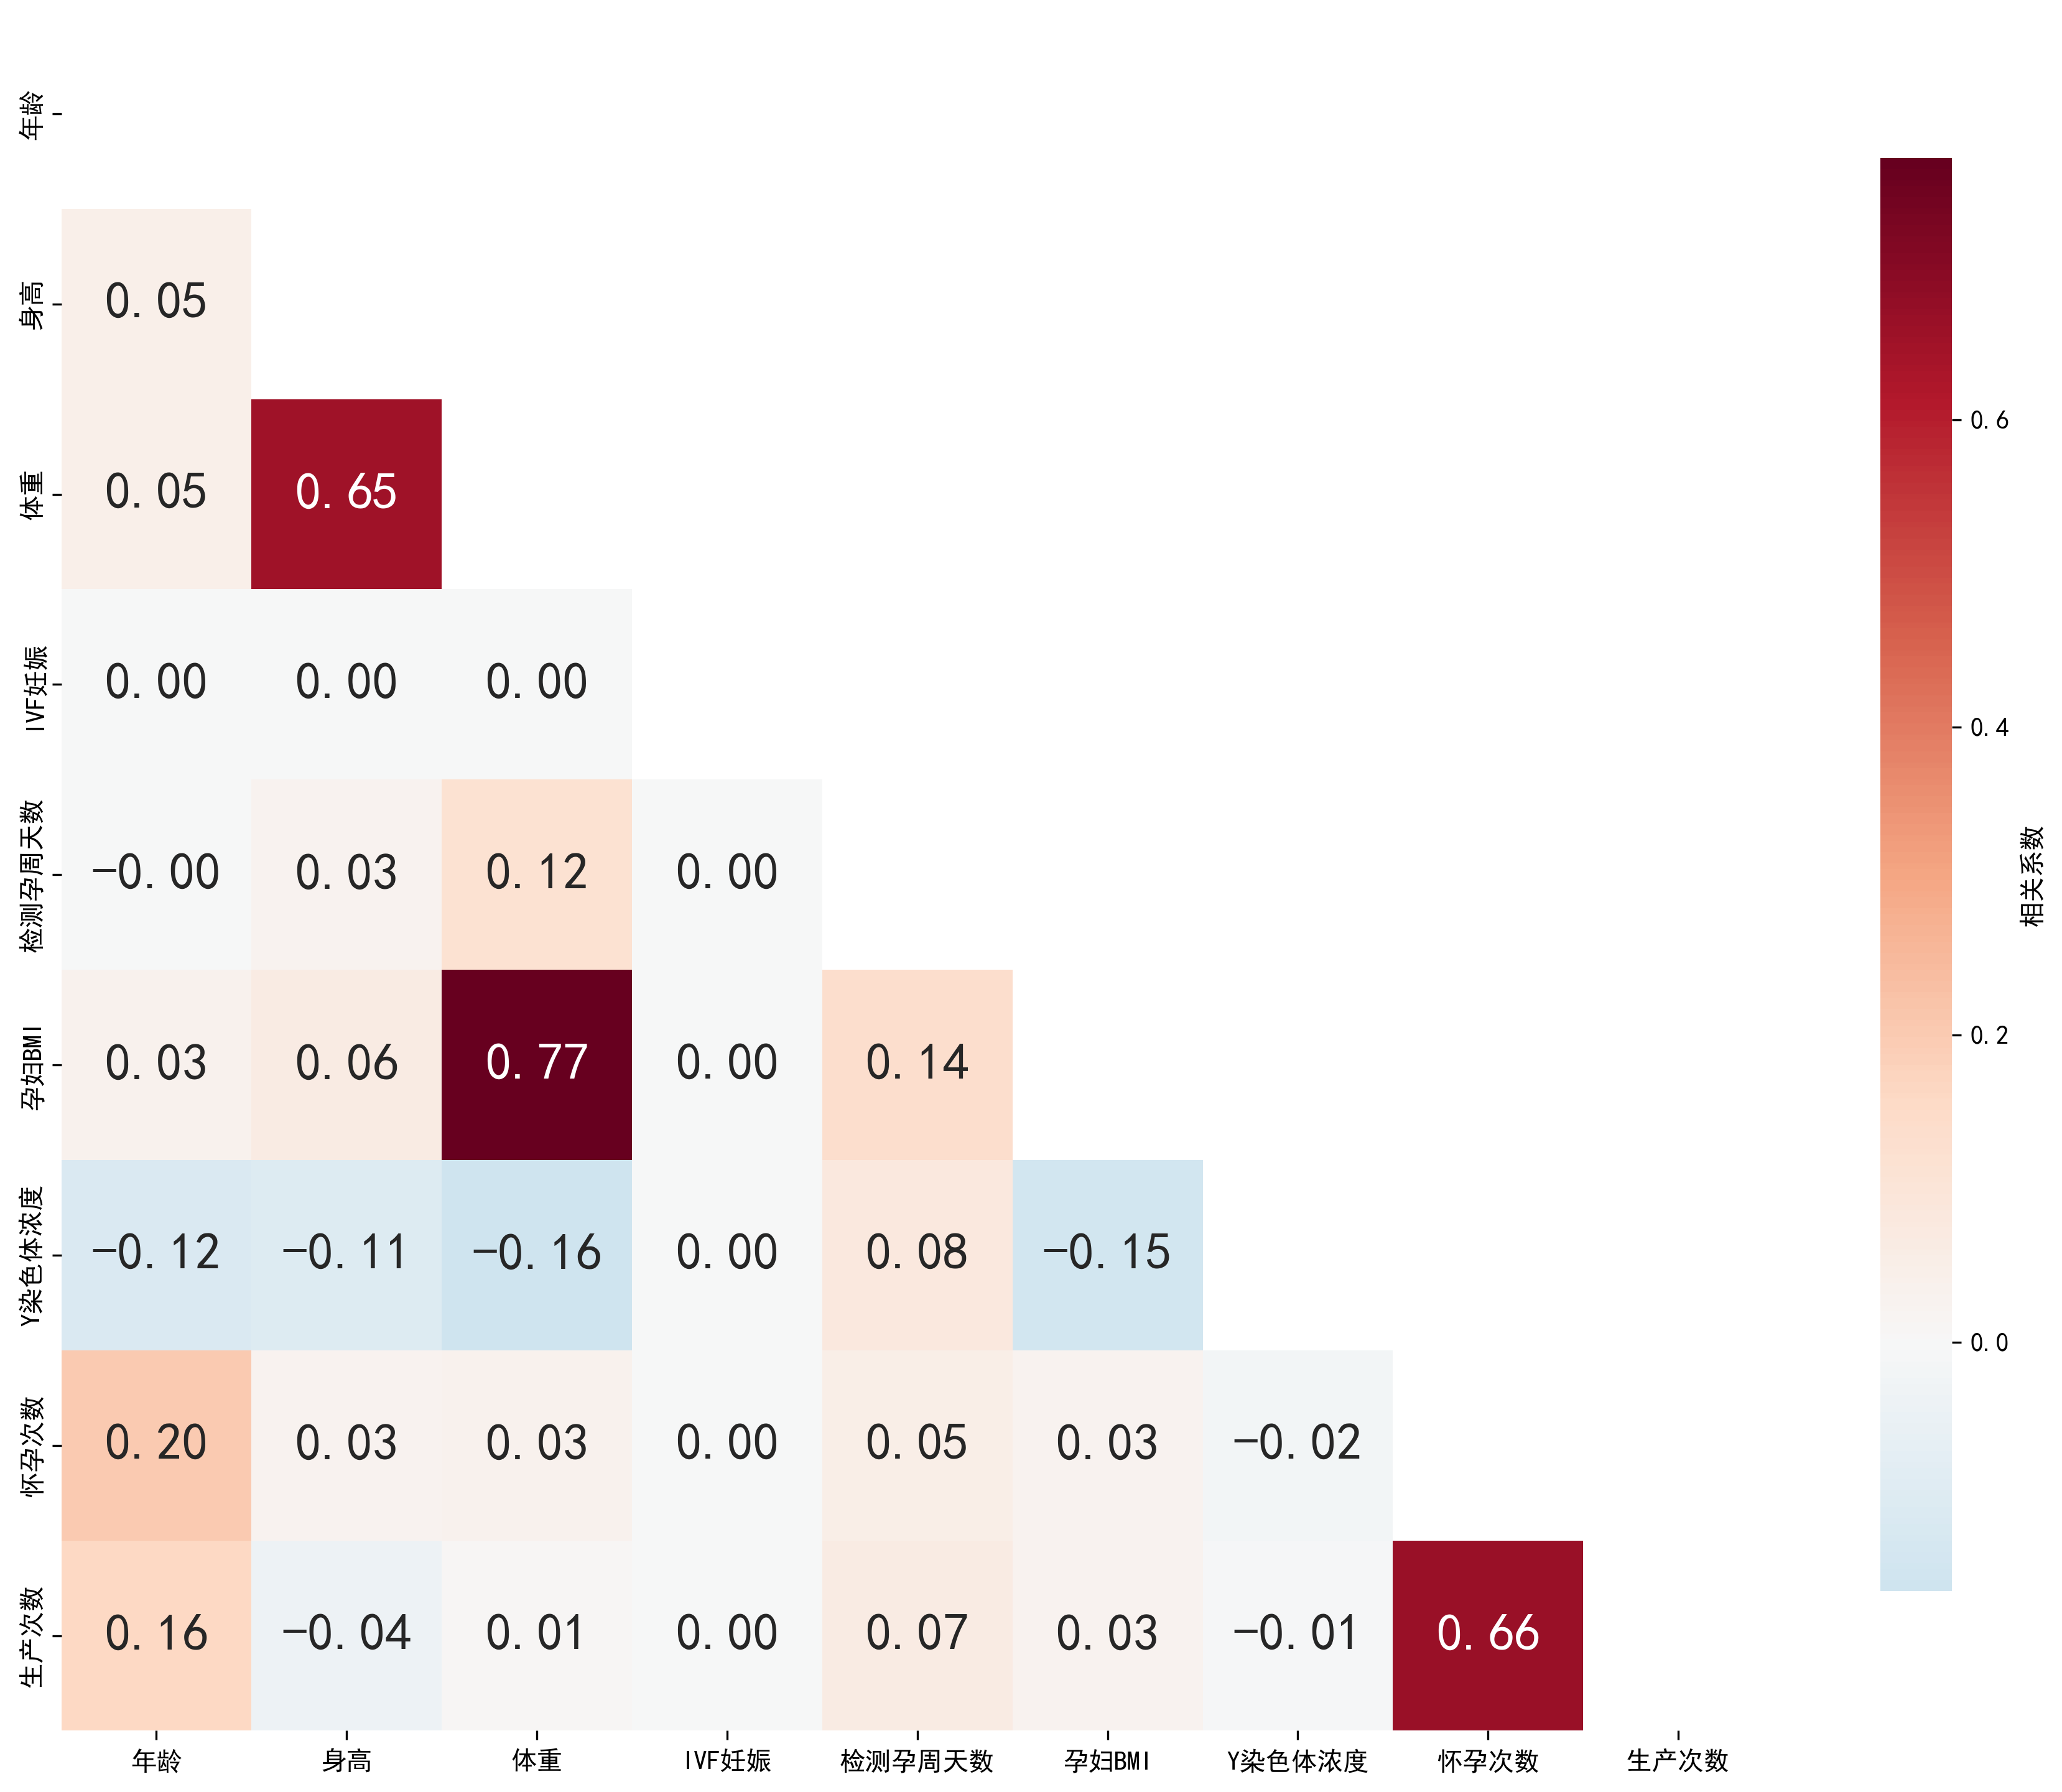
\includegraphics[width=0.7\textwidth]{figures/spearman5.png} 
		\caption{Y染色体相关系数分析图}
		\label{Y染色体相关系数}
	\end{figure}
	重点关注与Y染色体浓度存在相关性的数据。从图中可以看出,与Y染色体浓度相关性相对较高的影响因素有
	年龄、身高、体重、孕妇BMI和检测孕周天数。




	\begin{figure}[H]
		\centering
		\subcaptionbox{Y-BMI散点图\label{Y-BMI散点图}}
		{\includegraphics[width=.45\textwidth]{figures/Y-BMI散点图.png}}
		\hfill % 让两个子图尽可能分开
		\subcaptionbox{Y-天数散点图\label{Y-天数散点图}}
		{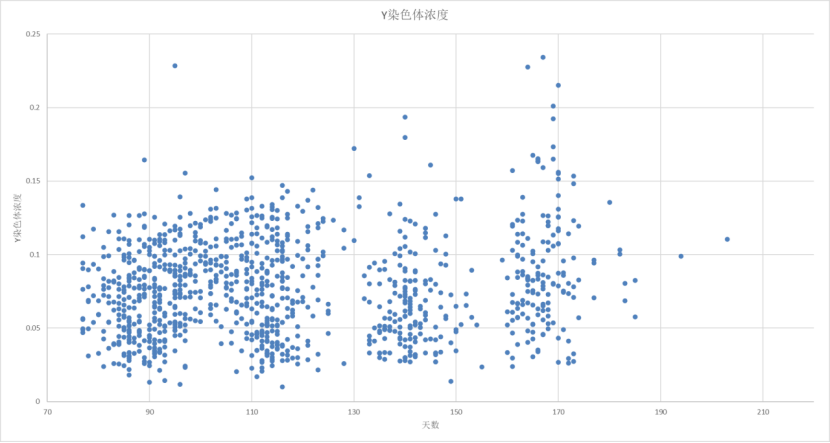
\includegraphics[width=.45\textwidth]{figures/Y-天数散点.png}}
		\caption{Y染色体浓度相关分析}
		\label{fig:Y染色体浓度与其他数据}
	\end{figure}



	绘制Y染色体浓度的分布直方图,观察分布直方图,发现Y染色体浓度分布近似于正态分布。通过Q-Q图进行检验
	可近似认为Y染色体浓度分布符合正态分布。
	\begin{figure}[ht]
		\centering
		\subcaptionbox{Y染色体浓度分布直方图\label{Y染色体浓度分布直方图}}
		{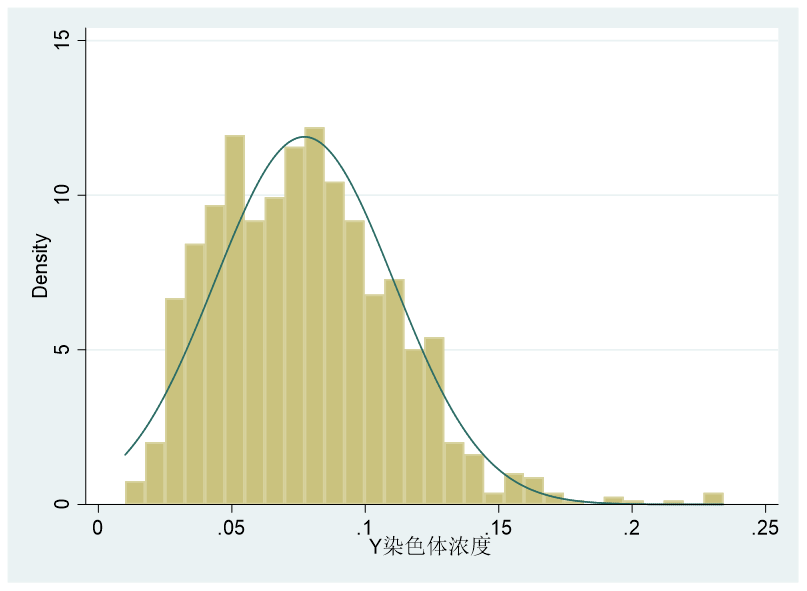
\includegraphics[width=.45\textwidth]{figures/Y染色体浓度分布.png}}
		\hfill % 让两个子图尽可能分开
		\subcaptionbox{Y染色体浓度的正态Q-Q图\label{Y染色体浓度的正态Q-Q图}}
		{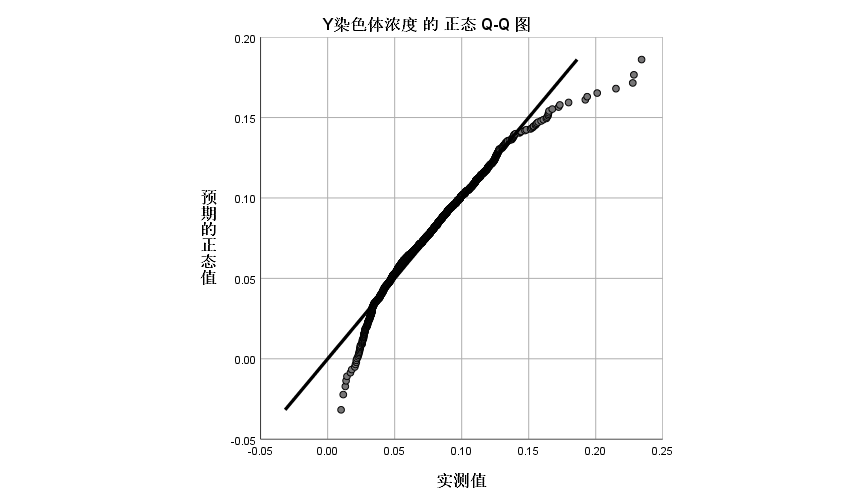
\includegraphics[width=.45\textwidth]{figures/Y染色体浓度正态.png}}
		\caption{Y染色体浓度数据分析}
		\label{fig:Y染色体浓度}
	\end{figure}


	\subsection{模型建立}
	考虑到数据集中存在多次检测和重复检测的数据,因此部分数据会嵌套相关联于同一个病人。且数据直接没有显著的线性相关性。
	我们采用广义可加模型对Y染色体浓度与孕妇身体数据的自变量进行建模。广义可加模型是广义线性模型的一种灵活扩展。将响应变量的期望值
	与预测变量之间的线性关系,转化为平滑的非线性关系。其中$\mu $为响应变量 ,$g(\mu)$ 为链接函数,$f_{j}(X_{j})$ 为平滑函数。

	\begin{equation}
	g(\mu) = \beta_0 + \sum_{j=1}^{p} f_{j}(X_{j})
	\end{equation}


	每个平滑函数 $f_{j}(X_{j})$ 都是一个未知形式的函数,它从数据中学习变量 $X_{j}$ 与响应变量之间的关系。
	利用链接函数将响应变量的分布与加性预测器联系起来。

	经过模型求解,IVF妊娠对Y染色体浓度没有显著影响,且其定性特性会影响其它变量的求解,因而我们选择剔除IVF妊娠,重新对模型进行求解。





	\subsection{模型求解}

	\begin{table}[H]
	\centering
	\caption{平滑项分析结果}
	\label{tab:smooth_terms}
		\begin{tabular}{lcccccc}
		\toprule
		平滑项 & Lambda & Rank & EDoF & P > x & p值 \\
		\midrule
		s(0) & 0.6 & 20 & 13.7 & 8.17e-10 & $<0.001$ \\
		s(1) & 0.6 & 20 & 11.6 & 4.18e-03 & $<0.001$ \\
		s(2) & 0.6 & 20 & 12.0 & 1.11e-16 & $<0.001$ \\
		s(3) & 0.6 & 20 & 9.6 & 1.06e-12 & $<0.001$ \\
		s(4) & 0.6 & 20 & 1.9 & 2.30e-01 & 0.1347 \\
		s(5) & 0.6 & 20 & 2.7 & 7.80e-01 & 0.3541 \\
		intercept & & 1 & 0.0 & 1.89e-15 &      \\
		\bottomrule
		\end{tabular}
	\end{table}





	
	
	

	
	\subsection{求解结果与分析}
	
	\begin{figure}[ht]
		\centering
		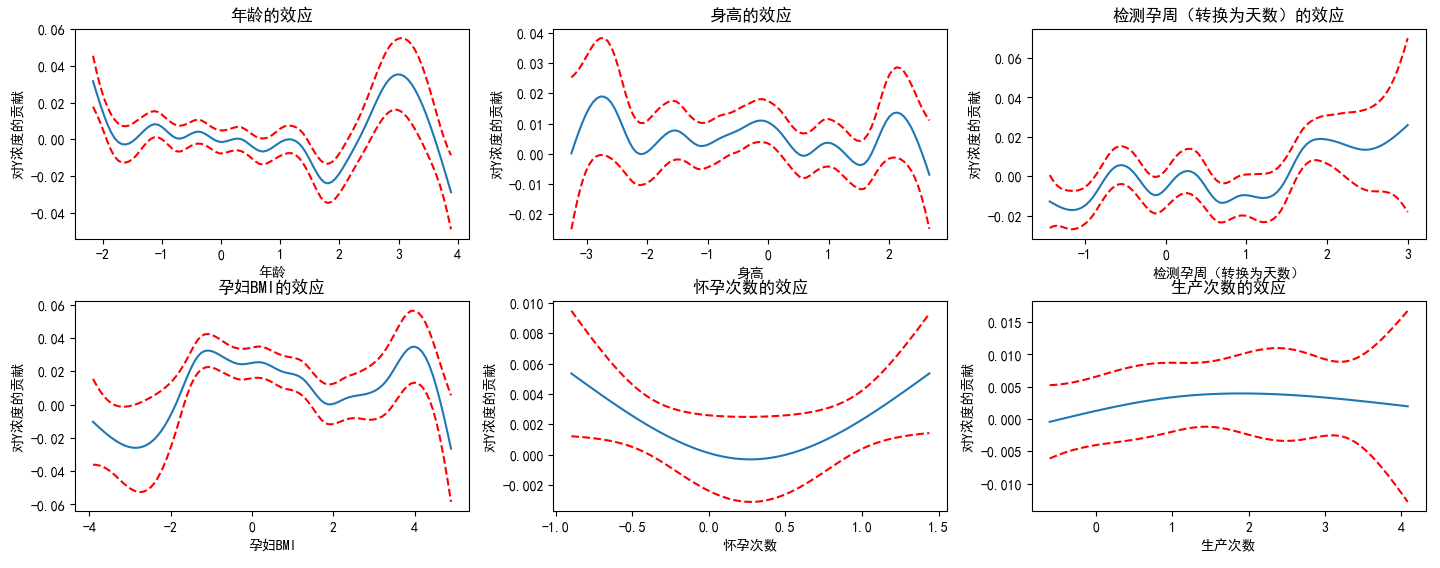
\includegraphics[width=0.7\textwidth]{figures/广义可加结果.png} 
		\caption{广义可加模型拟合结果图}
		\label{广义可加结果}
	\end{figure}

	这个GAM模型揭示了数据中存在复杂的非线性模式。
	
	首先,对于EDoF(自由度)指标,年龄、身高、检测孕周天数求解得到的EDoF都较大,说明这些指标都与Y染色体浓度存在复杂的非线性关系,孕妇BMI的EDoF最接近1,说明孕妇BMI相对于其它指标而言,与Y染色体浓度具有更强的线性相关性,而怀孕次数和生产次数的EDoF较小,说明模型难以捕捉到其与Y染色体浓度的响应关系,这与我们Spearman相关性检验的结果相近。

	其次,对于变量的显著性分析,年龄、身高、检测孕周天数、孕妇BMI均满足p<0.001,对Y染色体浓度具有显著的影响,而怀孕次数和生产次数p值均较高对Y染色体浓度的影响并不显著。在变量各自的显著性分析下,前者对于Y染色图浓度由显著的影响,我们可以认为这个加性模型是显著的。

	综上所述,本次分析揭示了年龄、身高、检测孕周天数和孕妇BMI对Y染色体浓度的显著影响和它们之间的相关性,为后续对Y染色体浓度达标时间的研究奠定了基础。

	
	%%%%%%%%%%%%%%%%%%%%%%%%%%%%%%%%%%%%%%%%%%%%%%%%%%%%%%%%%%%%%
	\section{问题二的模型建立与求解}

	问题2核心要求是对男胎孕妇的BMI进行合理分组,给出每组对应的最佳NIPT检测时点,使得孕妇因延迟发现胎儿
	异常而产生的潜在风险最小化。在进行NIPT检测时,一般要求Y染色体浓度达到或超过4\%,才认为检测结果是准确的。
	临床证明,孕妇BMI是影响Y染色体浓度的主要因素。BMI通过影响孕妇BMI指数从而影响最早检测达标时间。而潜在风险
	与发现时间相联系,一般越晚发现,风险越高,介入治疗风险越大。最后需要考虑检测误差对结果的影响。数据集中的检测结果并非连续时间段,对应
	达标时间可能并不准确。

	首先需要根据BMI,对孕妇进行分组。由问题一可知,BMI对Y染色体浓度的影响,是一个复杂的非线性关系。因此我们难以采用一些线性方法对BMI进行判断分组。
	考虑到这个特点,我们采用决策树进行分组处理。利用决策树算法来最大化数据组间差异,最小化数据组内差异,利用数据驱动,自动找到连续变量BMI的最佳
	分隔点,获得影响达标时间的关键BMI阈值。

	考虑到实际中,孕妇一般按照固定周期进行孕检。如一个月进行一次体检。因此在给定数据集中存在大量左删失,右删失的情况。我们难以确定孕妇Y染色体浓
	度为4\%的确切时间点。如果采用传统回归方法处理该问题,处理效果较差。因此我们考虑使用生存模型对每组的最佳NIPT检测时点进行求解。最大限度的
	利用数据集中的部完整数据。


	\subsection{问题二的思路分析}

	\subsection{数据预处理}

	\subsubsection{有效数据筛选}

	对低质量样本进行剔除。要求高质量样本满足以下条件:
	\begin{itemize}[itemindent=2em]
		\item \textbf{原始读段数 $\geq 3000000$:} 意义
		\item \textbf{唯一比对读段数 $\geq 2500000$:} 意义
		\item \textbf{参考基因组上比对的比例 $\geq 75\%$:} 意义
		\item \textbf{重复读段比例 $\leq 5\%$:} 意义
		\item \textbf{被过滤掉读段数比例 $\geq 3000000$:} 意义
		\item \textbf{GC 含量偏离在 0.4-0.6 范围内不大,即认为正常:} 
	\end{itemize}

	\subsubsection{目标数据获取}


	目标数据获取:


	\subsection{决策树模型建立}

	用回归树把BMI空间按对预测W首次达标时间进行有区间划分,

	\subsubsection{依据BMI进行分组}

	以孕妇的 BMI 为分组变量,通过 回归树(DecisionTreeRegressor) 学习数据中“BMI与
	达标孕周时间之间的非线性关系,根据 最小化组内方差 的原则,自动找到 BMI 的分裂点,把
	孕妇划分成不同的 BMI 区间。每个叶节点就是一个 BMI 分组。

	\subsubsection{选择最佳NIPT时点}



% ==== 事件指示 ====

	\begin{equation*}  
		\delta_i = 1 - c_i
	\end{equation*}

% ==== 节点样本集合 ====
	\begin{equation*}
		\mathcal{D}_j = \{(X_i,T_i,\delta_i)\in\mathcal{D}:\ X_i\in I_j\}
	\end{equation*}

% ==== 树划分左右子集 ====
	\begin{equation*}
		L(s)=\{i: X_i\le s\},\qquad R(s)=\{i: X_i> s\}
	\end{equation*}

% ==== 最优分割点 ====
	\begin{equation*}
		s^*=\arg\min_s\ \sum_{i\in L(s)}(T_i-\bar T_{L})^2 + \sum_{i\in R(s)}(T_i-\bar T_{R})^2
	\end{equation*}

% ==== 区间递归关系 ====
	\begin{equation*}
		I_{j,\text{left}} = (l_j,\,\theta_j],\qquad I_{j,\text{right}} = (\theta_j,\,u_j)
	\end{equation*}

% ==== 样本分配判据 ====
	\begin{equation*}
		i\in \mathcal{D}_j \;\;\Leftrightarrow\;\; l_j < X_i \le u_j
	\end{equation*}









	\subsection{基于决策树的蒙特卡洛模拟}


	
	\subsubsection{依据BMI进行分组}

	分组依据是 BMI,采用 决策树(CART),依据“信息增益”或“基尼指数”来分裂节点。
	具体实现:
	首先,初分组使用 BMI 单变量建树去区分事件是否发生;
	然后,对分组进行两层筛选(说清楚为什么这么筛):
	样本数量约束:每组满足数据总量在[20,200],分析理由;
	BMI区间间隔约束:若两个子组BMI平均值间隔<2,认为其分析理由,则不拆分子组,保持合并;


	\subsubsection{选择最佳NIPT时点}

	首先,对每个分组,计算Kaplan–Meier 生存函数,统计累计达标率,并定义综合评价
	模型,步骤和使用参数与问题二方法一一致;然后,若向量两组的最优时点差异太小,通
	过移动BMI边界调整分组,直到差异收敛。

% ==== Kaplan–Meier 生存函数 ====
	\begin{equation*}
		\hat S_j(t) = \prod_{t_k \le t} \Big(1 - \tfrac{d_k}{n_k}\Big)
	\end{equation*}

% ==== 覆盖率 ====
	\begin{equation*}
		C_j(t) = 1 - \hat S_j(t)
	\end{equation*}



% ==== 时间归一化 ====
	\begin{equation*}
		r(t) = \frac{t-t_{\min}}{t_{\max}-t_{\min}}
	\end{equation*}

% ==== 目标函数 ====
	\begin{equation*}
		f_j(t)=\alpha\, C_j(t) + (1-\alpha)\big(1-r(t)^p\big)
	\end{equation*}
	
% ==== 最佳时点 ====
	\begin{equation*}
		t_j^* = \arg\max_{t \in \mathcal{T}_j} f_j(t)
	\end{equation*}


\begin{itemize}
    \item 其中 $\text{Coverage}(t)$ = 截止孕周 $t$ 已达标的比例(越大越好,表示检测成功率高)。
    \item 第二项是"风险递减函数",孕周越大,风险越高,所以值越小。
    \item 参数 $\alpha$(如 0.4)控制两者权重。
    \item \textbf{筛选原则}: 在 70-196 天(10-28 周)区间内,找到使 $f(t)$ 最大的孕周作为 \textbf{最佳检测时点}。
\end{itemize}


最后,在节点j上选择最优时点:{对应公式}其中 $T_j$为被用于枚举的时间点集合(代码中使用 Kaplan–Meier 返回
的格点 times,也可以改为更细的格点并用插值)。若满足条件的时间点为空,代码退化到取最后观测时间.





\subsubsection{分析误差对结果的影响}

在建模过程中,我们假设Y染色体浓度的观测值存在测序误差。该误差来源于测序平台的噪声、样本提取的批次效应及个体差异。
若直接使用观测值来判断“首次达标时间”,可能导致阈值附近的判断偏差,从而影响分组与最佳检测时点的推荐。
经统计检验我们发现观测误差具有更厚的尾部,更符合t 分布特征。这意味着极端偏差出现的概率更高。
为此,我们采用蒙特卡洛模拟方法。

\begin{enumerate}
    \item 对每个孕妇样本,设实际观测值为 $\mu$,误差项 $\epsilon \sim t_\nu(0, \sigma)$,其中自由度 $\nu$ 与尺度参数 $\sigma$ 由样本拟合得到。于是模拟观测值为
    \[
    \tilde{Y} = \mu + \epsilon, \quad \epsilon \sim t_\nu(0, \sigma).
    \]
\end{enumerate}

进行500次重复采样,每次从上述误差分布中独立抽取误差值,叠加到实际观测值,计算出模拟观测值;
在不改变BMI分组的前提下,利用模拟观测值重复最佳时点选择过程,获得受检查误差影响的选择结果。

然后使用蒙特卡洛模拟,对观测到的Y染色。



	\section{问题三的模型建立与求解}

	\subsection{模型建立}
	\subsection{模型求解}
	为求解上述模型,我们设计了如下步骤:
	
	\begin{description}
		\item[Step 1:] 数据预处理...
		\item[Step 2:] 利用 MATLAB/Python 实现...算法...
		\item[Step 3:] 结果后处理与可视化...
	\end{description}


















	\section{问题四的模型建立与求解}

	以女胎孕妇的21号染色体,18号染色体,13号染色体非整倍体为判定结果。
	分析胎儿是否异常。这是一个典型的二分类问题,正常胎儿和异常胎儿。逻辑回归
	较适于处理这类问题,通过sigmoid函数将线性组合的输出映射到$[0,1]$区间,表示异常的概率。
	当输出概率大于0.5可判定异常,否则为正常。
	
	问题4需要综合考虑多个因素,包括多条染色体
	的Z值,GC含量,读段数,BMI等。利用逻辑回归可以轻松纳入多个影响因素,并通过训练数据估计
	每个变量的权重,从而构建一个综合判定模型,从而达到捕捉多个因素之间的复杂关系。

	逻辑回归模型中的系数提供了每个特征对异常概率的影响方向和大小。例如,正系数表示该特征增加
	异常概率,负系数表示减少异常概率。这种可解释性有助于在医学领域解释影响因素,并进行进一步研究。











	\subsection{数据预处理}
	剔除质量不合格剔除质量不合格样本、对变量进行标准化,虚拟变量化、标记疑似异
	常样本,为后续建模提供干净一致的数据集。

	\subsubsection{标记高质量样本}

	对低质量样本进行剔除。要求高质量样本满足以下条件:
	\begin{itemize}
		\item 原始读段数 >= 3000000
		\item 唯一比对读段数 ≥ 2,500,000
		\item 参考基因组上比对的比例 ≥ 75\%
		\item 重复读段比例 ≤ 5\%
		\item 被过滤掉读段数比例 ≤ 5\%
		\item GC 含量偏离在 0.4-0.6 范围内不大,即认为正常.
	\end{itemize}

	\subsubsection{异常标记}

	若任一染色体的$|Z|>3$或 AB 标注异常,则标为疑似异常样本(值=1),否则为0.


	\subsubsection{变量处理}

	将连续变量做标准化,非连续变量和分类变量转换为虚拟变量。虚拟变量转换可见\cref{量化处理}。

	

	\subsection{共线性诊断与显著变量筛选}

	\subsubsection{线性回归共线性诊断}
	计算多个模型步骤中各变量的Beta,t,显著性(P值),偏相关,容差与方差碰撞因子











	18号染色体的Z值,ZX染色体浓度,Z孕妇BMI以及13号和21号染色体的GC含量是与“胎儿是否异常”显
	著相关的因素。其中13号染色体的GC含量的容差为0.048,21号染色体的GC含量的容差为0.047。
	均小于0.1。同时,13号染色体的GC含量的VIF为20.721,21号染色体的GC含量的VIF为21.1,均远大于10
	我们认为其存在多重共线性,相互高度相关。其他变量的VIF接近1,可认为不存在多重共线性。



	\subsubsection{LASSO回归}
	进行共线性诊断后,仍存在大量的影响因素,不利于建立逻辑回归模型。因此使用LASSO回归进行变量选择。
	提高模型的泛化性,减少模型受到个体差异数据的影响。




	选中的lambda最终产生11个非零系数。其中Z生产次数,pregent1,pregent3,born3的系数较小,其对模型
	的贡献值较低,可以舍弃这四个影响因素。保留其中系数相对较大的因素:13号染色体的Z值、18号染色体的
	Z值、Z年龄、Z孕妇BMI、Z唯一比对的读段数、ZX染色体浓度、Z13号染色体GC含量等。


	\subsubsection{逐步逻辑回归}
	使用向前逐步法输入变量,逐步纳入显著变量,最终纳入的变量顺序与结果:
	\begin{description}
		\item[Step 1:] 输入18号染色体的Z值(显著)
		\item[Step 2:] 加入ZX染色体浓度(显著)
		\item[Step 3:] 加入Z13号染色体的GC含量(显著)
		\item[Step 4:] 加入Z孕妇BMI(显著) 
	\end{description}


	最终建议的候选变量:18号染色体的Z值、ZX染色体浓度、Z13号染色体的GC含量、Z孕妇BMI
	Z年龄($ p \approx 0.066 $)有近显著性,可选择性纳入,查看模型是否得到改善。
	13号染色体的 Z 值:在最后一步 p=0.065(>0.05),可能因与 18 号 Z 值共线而被替代,进行剔除处理。
	Z唯一比对的读段数:p=0.076。p值较小,显著性较低,进行剔除处理。

	\subsection{模型建立与求解}

	将逐步筛选后的5个变量,(@18号染色体的Z值,ZX染色体浓度,Z@13号染色体的GC含量,Z孕妇BMI,Z年龄)一次
	性输入,分别设为$\displaystyle x_{1}\sim x_{5}$,建立如下模型,并对模型性能进行多项评估。

	\begin{equation*}
	\label{logit}
	\text{Logit}(P) = 2.106 + 0.925 \cdot x_{1} - 0.823 \cdot x_{2} + 0.442 \cdot x_{3} - 0.148 \cdot x_{4} - 0.202 \cdot x_{5}
	\end{equation*}

	\begin{equation*}
	P = \frac{1}{1 + e^{-\mathrm{Logit}(P)}}
	\end{equation*}


	利用ROC曲线进行阈值选择。确定阈值为0.1337625
	\begin{figure}[ht]
		\centering
		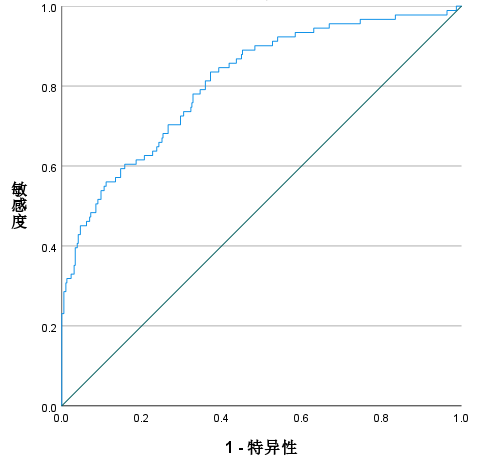
\includegraphics[width=0.3\textwidth]{figures/ROC曲线.png} 
		\caption{ROC曲线图}
		\label{ROC曲线}
	\end{figure}

	当$P\geq0.1337625 $,认为异常。


	回归系数


	默认阈值 $0.5$ 下的分类表显示:

	对阴性样本(是否异常$=0$)预测正确率非常高 $97.2\%$(但阴性样本占比大)。对阳性样本(是否异常$=1$)预测正确率低,
	仅 $33.0\%$ $\rightarrow$ 表明模型对异常(阳性)的敏感性差。总体准确率 $84.9\%$,但被类别不平衡掩盖(阴性远多于
	阳性)。

	

	\begin{table}[!ht]
		\centering
		\caption{模型检验}
		\label{模型检验}
		\begin{tabular}{|l|l|l|}
		\hline
			模型检验 & 结果 & 解释 \\ \hline
			Omnibus检验 & $\chi^2 = 112.924$, $p < 0.001$ & 整体模型显著优于空模型 \\ \hline
			Nagelkerke & $R^2 = 0.338$ & 模型可解释约 34\% 的变异 \\ \hline
			Hosmer-Lemeshow 拟合优度检验 & $\chi^2 = 8.999$, $p = 0.342$ → $p > 0.05$ & 模型拟合尚可,无明显差异\\ \hline
		\end{tabular}
	\end{table}





	
	
	\subsection{模型优化}

	为探索变量间复杂的交互效应,我们基于生物学常识引入了‘年龄与BMI的交互项’($Z_{\text{年龄}} \times Z_{\text{孕妇BMI}}$)进行测试。结果表明,
	该交互项效应不具有统计学意义($p=0.112$)。根据模型简洁性原则,我们最终保留了不含交互项的初始模型,该模型具有更佳的稳
	定性和可解释性

	加了年龄的平方之后的模型结果显示,$Z_{\text{年龄}}$和$Z^{2}_{\text{年龄}}$两个变量都变得高度显著($p=0.000$),这种“负的线性
	项 + 正的二次项”的组合,清晰地表明了一种“U型”关系:胎儿异常的风险先随着孕妇年龄的增加而下降,到达一个最低点(谷底)后
	,又随着孕妇年龄的继续增加而上升.
	已知数据:
	\begin{itemize}
		\item 	$Z_{\text{年龄}} $ 的系数  $B_{1} = -4.847$
		\item 	$Z^{2}_{\text{年龄}}$ 的系数 $B_{2} = 4.729$
		\item 	原始年龄的均值 $\bar{y} = 29.92 $岁
		\item 	原始年龄的标准差 $S = 4.303 $岁
	\end{itemize}

	待求值:风险最低的实际年龄

	通过Z值拐点即$Y_{Z}$转换计算:
	\begin{equation}
	Y_{Z} = -\frac{B_1}{2 \times B_2} = -\frac{-4.847}{2 \times 4.729} = \frac{4.847}{9.458} \approx 0.512
	\end{equation}

	转换为实际年龄$Y$:

	\begin{equation}
	\text{Y} = \bar{y} + (Y_{\text{Z}} \times S) = 29.92 + (0.512 \times 4.303)
	\end{equation}

	通过二次函数直接计算

	计算系数 $a$ 和 $b$:
	\begin{align}
	a &= \frac{B_2}{S^2} = \frac{4.729}{(4.303)^2} \approx \frac{4.729}{18.516} \approx 0.255 \\
	b &= \frac{B_1 - 2 \times B_2 \times \frac{\bar{y}}{S}}{S} = \frac{-4.847 - 2 \times 4.729 \times \frac{29.92}{4.303}}{4.303} \approx -16.41
	\end{align}

	计算拐点:
	\begin{align}
	Y = -\frac{b}{2a} = -\frac{-16.41}{2 \times 0.255} = \frac{16.41}{0.51} \approx 32.176
	\end{align}

	最终结论
	两种方法的计算结果高度一致($32.12$ vs $32.18$),确认了结果的可靠性。

	在研究人群中,怀有异常女胎的风险最低的孕妇年龄为  $\thickapprox 32.2$ 岁。

	这是一个非常重要的U型关系:

	\begin{itemize}
	\item 轻孕妇($<32.2$岁):胚胎的风险随年龄增加而下降
	\item 最佳年龄( $32.2$岁左右):胚胎的风险达到最低点
	\item 高龄孕妇($>32.2$岁):胚胎的风险随年龄增加而上升
	\end{itemize}

	这一发现揭示了孕妇年龄与异常风险之间复杂的非线性关系,为临床咨询和风
	险评估提供了更精确的科学依据。

	增加年龄平方项后的Logistic回归结果
	\begin{equation*}
	\label{logit2}
	\text{Logit}(P) = 2.874 + 0.955 \cdot x_{1} - 0.887 \cdot x_{2} + 0.470 \cdot x_{3} - 0.476 \cdot x_{4} - 4.847 \cdot x_{5} +4.729 \cdot x^{2}_{5}
	\end{equation*}


	\subsection{结果分析}

	\begin{table}[H]
	\centering
	\caption{训练集与测试集混淆矩阵对比}
	\label{训练集与测试集混淆矩阵对比}
		\begin{tabular}{|c|c|c|c|c|}
		\hline
		\multirow{2}{*}{数据集} & \multirow{2}{*}{实测 \textbackslash 预测} & \multicolumn{2}{c|}{预测类别} & \multirow{2}{*}{行总计} \\ \cline{3-4}
		& & 正常 (0) & 异常 (1) & \\ \hline
		\multirow{4}{*}{训练集} & 真实正常 (0) & 374 (TN) & 13 (FP) & 387 \\ \cline{2-5}
		& 真实异常 (1) & 57 (FN) & 34 (TP) & 91 \\ \cline{2-5}
		& 列总计 & 431 & 47 & 478 \\ \hline
		\multirow{4}{*}{测试集} & 真实正常 (0) & 100 (TN) & 5 (FP) & 105 \\ \cline{2-5}
		& 真实异常 (1) & 10 (FN) & 10 (TP) & 20 \\ \cline{2-5}
		& 列总计 & 110 & 15 & 125 \\ \hline
		\end{tabular}
	\end{table}


	\begin{table}[H]
	\centering
	\caption{训练集与测试集性能指标对比}
	\label{训练集与测试集性能指标对比}
	\renewcommand{\arraystretch}{2.2} % 增加行高
		\begin{tabular}{|l|c|c|c|}
		\hline
		\multicolumn{1}{|c|}{\textbf{指标}} & \multicolumn{1}{c|}{\textbf{计算公式}} & \multicolumn{1}{c|}{\textbf{训练集}} & \multicolumn{1}{c|}{\textbf{测试集}} \\ 
		\hline
		总体准确率 & $\dfrac{TP + TN}{TP + TN + FP + FN}$ & 85.4\% & 88.0\% \\ 
		\hline
		敏感性(召回率) & $\dfrac{TP}{TP + FN}$ & 37.4\% & 50.0\% \\ 
		\hline
		特异性 & $\dfrac{TN}{TN + FP}$ & 96.6\% & 95.2\% \\ 
		\hline
		精确率 & $\dfrac{TP}{TP + FP}$ & 72.3\% & 66.7\% \\ 
		\hline
		F1-Score & $2 \times \dfrac{Precision \times Recall}{Precision + Recall}$ & 49.4\% & 57.2\% \\ 
		\hline
		\end{tabular}
	\end{table}

	模型在训练集上表现出高特异性(96.6\%)和高精确率(72.3\%),但敏感性较
	低(37.4\%),这意味着模型非常保守,漏诊了很多异常案例,但一旦预测为异
	常,可信度很高。
	模型在未知数据上表现甚至优于训练集!总体准确率和敏感性都有所提升。特异性
	依然极高(95.2\%),而敏感性提升至50\%,这是一个重大的改善。

	预测集的所有关键指标都与训练集相当甚至更好,证明模型没有过拟合,具有很强
	的泛化到新数据的能力。
	预测集上50\%的敏感性是一个重要成果。它意味着模型能识别出一半的真实异常病
	例,这对于初步筛查来说具有重要价值,可以大大减少漏诊。
	95\%以上的特异性意味着模型“虚惊一场”的假警报很少,这可以避免给大量孕妇带
	来不必要的心理压力和进一步的创伤性检查。
	这是一个非常实用的筛查模型。它的特点是“宁可漏诊,也不错报”,但即便如此,也
	成功捕捉到了50\%的异常案例,为高风险人群的早期发现提供了有力工具。








	
	% ... 后续问题类似 ...

	%%%%%%%%%%%%%%%%%%%%%%%%%%%%%%%%%%%%%%%%%%%%%%%%%%%%%%%%%%%%%
	\section{模型的评价与推广}
	\subsection{模型的优点}
	\begin{itemize}[itemindent=2em]
		\item 优点1:模型结构简洁,物理意义明确。
		\item 优点2:算法效率高,求解速度快。
		\item 优点3:模型具有较好的通用性,可推广至...
	\end{itemize}
	\subsection{模型的缺点}
	\begin{itemize}[itemindent=2em]
		\item 缺点1:假设条件较强,在...情况下可能失效。
		\item 缺点2:未考虑...因素,与实际情况存在一定偏差。
	\end{itemize}



	\begin{lemma}
		这是一个引理...
	\end{lemma}
	\begin{definition}
		这是一个定义...
	\end{definition}
	
	%%%%%%%%%%%%%%%%%%%%%%%%%%%%%%%%%%%%%%%%%%%%%%%%%%%%%%%%%%%%%
	%% 参考文献
	% 建议:最终提交时删除 \nocite{*}
	% \nocite{*}
	\bibliographystyle{gbt7714-numerical} % 引用格式,符合国标
	\bibliography{ref} % 你的 .bib 文件名,这里假设是 ref.bib
	
	\newpage
	%%%%%%%%%%%%%%%%%%%%%%%%%%%%%%%%%%%%%%%%%%%%%%%%%%%%%%%%%%%%%
	%% 附录
	\begin{appendices}
		\section{支撑材料列表}
		\begin{table}[H]
			\centering
			\caption{附录文件列表}
			\label{tab:文件列表}
			\begin{tabularx}{\textwidth}{LL}
				\toprule
				文件名 & 功能描述 \\
				\midrule
				q1.m & 问题一核心 MATLAB 程序代码 \\
				q2.py & 问题二 Python 求解程序 \\
				data.xlsx & 本文使用的原始数据与处理结果 \\
				\bottomrule
			\end{tabularx}
		\end{table}
		
		\section{核心代码}
		\noindent\textbf{问题一 MATLAB 代码 (q1.m)}
		\lstinputlisting[language=matlab]{code/q1.m}
		
		\noindent\textbf{问题二 Python 代码 (q2.py)}
		\lstinputlisting[language=python]{code/q2.py}
		
	\end{appendices}
	
\end{document}